\documentclass[12pt, aspectratio=169]{beamer}
 \usepackage{listings}
\usepackage{minted}
\usepackage{tikz}
\usetikzlibrary{calc}

\useoutertheme{infolines}

\definecolor{secinhead}{RGB}{249,196,95}
\definecolor{foot}{RGB}{70,67,67}
\definecolor{footfg}{RGB}{198,155,73}
\definecolor{titlebg}{RGB}{51,51,51}

\setbeamercolor{secsubsec}{fg=secinhead,bg=black}
\setbeamercolor{frametitle}{fg=secinhead,bg=titlebg}
\setbeamercolor{footline}{fg=footfg,bg=foot}
\setbeamercolor*{title}{fg=secinhead,bg=titlebg}


% standard enumeration
\setbeamertemplate{enumerate items}{(\arabic{enumi})}

% default itemize
\setbeamertemplate{itemize items}[circle]

% transparency
\setbeamercovered{transparent=9}


\setbeamertemplate{headline}
{
  \leavevmode%
  \hbox{%
  \begin{beamercolorbox}[wd=\paperwidth,ht=4.5ex,dp=3.5ex]{secsubsec}%
    \raggedright
    \hspace*{3em}%
    {\sffamily\small\color{secinhead}\thesection.~\insertsection\hfill\insertsubsection}%
    \hspace*{2em}%
  \end{beamercolorbox}%
  }%
}


\setbeamertemplate{footline}
{%
  \vspace{.1em}
  \leavevmode%
  \hbox{%
  \begin{beamercolorbox}[wd=\paperwidth,ht=1.2ex,dp=0.5ex]{footline}%
    \raggedright
    \hspace*{3em}%
    {\sffamily\scalebox{.7}{\color{secinhead}\insertauthor}\hfill\scalebox{.7}{\inserttitle}\hfill\scalebox{.7}{\insertframenumber/\inserttotalframenumber}}%
    \hspace*{2em}%
  \end{beamercolorbox}%
  }%
}



\setbeamertemplate{frametitle}
{\vskip-2pt
  \leavevmode
  \hbox{%
  \begin{beamercolorbox}[wd=\paperwidth,ht=2.2ex,dp=1ex]{frametitle}%
    \raggedright\hspace*{1.8em}\large\insertframetitle
  \end{beamercolorbox}
  }%
}


\setbeamertemplate{navigation symbols}{}


\graphicspath{
  {img/}
}


\begin{document}
\title{Workshop on Python Programming}  
\author{Bibek Gautam}
\date{\today} 

\begin{frame}[plain]
  \titlepage
\end{frame}
% \begin{frame}[plain]
%   \tableofcontents
% \ end{frame}



\section{Intro to Python} 
\frame{\frametitle{Why Python?} 
  \only<1>{
   \begin{figure}
\hspace{-4em}\centering   
\includegraphics[width=0.28\textwidth]{pythonlogo} 
   \end{figure}
 
  }
\only<2>{
  \begin{columns}
    \begin{column}{4cm}

   \begin{figure}[left]
   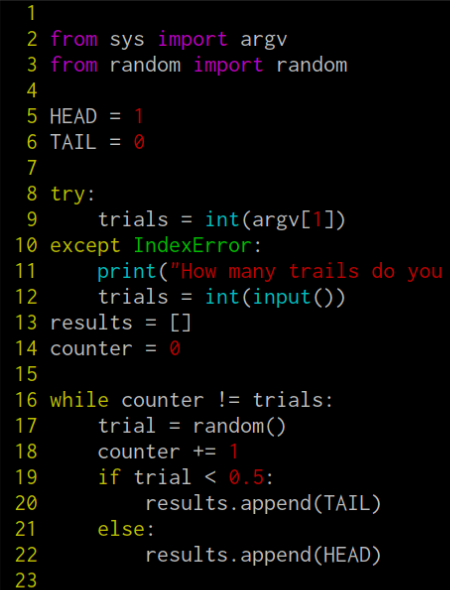
\includegraphics[scale=0.24]{python} 
    \caption{Python}
    \label{fig:py}
  \end{figure}
    \end{column}

    \begin{column}{5cm}
  \begin{figure}[left]
   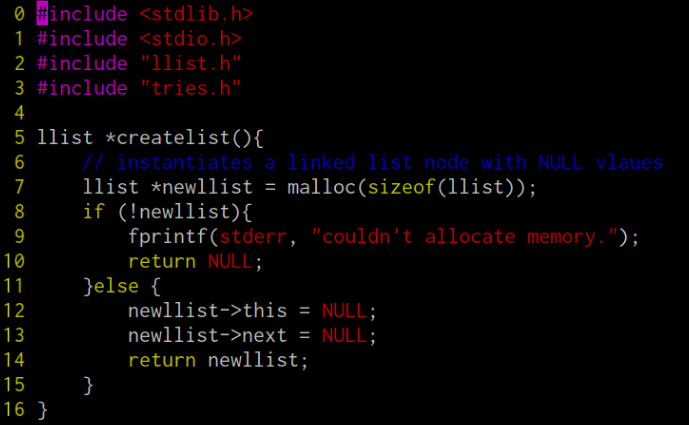
\includegraphics[scale=0.23]{c} 
    \caption{c}
    \label{fig:c}
  \end{figure}
    \end{column}
    
  \end{columns}
}
\only<3>{
  \begin{columns}
    \begin{column}{4cm}
   \begin{figure}
      \hspace{-4em}
   
\includegraphics[width=0.38\textwidth]{youtube}  \\ 
      \vspace{1em}
%\tikz[remember picture, overlay] \node[anchor=center] at ($(current page.center)-(1,1))$) {
\includegraphics[width=0.38\textwidth]{youtube} };
      \hspace{-4em}
   
\includegraphics[width=0.38\textwidth]{mozilla}  \\ 
      \vspace{1em}
      \hspace{-4em}
   
\includegraphics[width=0.38\textwidth]{dropbox} 
   \end{figure}
   \end{column}
    \begin{column}{4cm}
   \begin{figure}
      
\includegraphics[width=0.38\textwidth]{nasa}  \\ 
      \vspace{1em}
      
\includegraphics[width=0.38\textwidth]{bittorrent}  \\ 
      \vspace{1em}
      
\includegraphics[width=0.38\textwidth]{ibm} 
   \end{figure}
   \end{column}
   \end{columns}
 }
\only<4>{
  \begin{columns}
    \begin{column}{4cm}
   \begin{figure}
      \hspace{-4em}
   
\includegraphics[width=0.38\textwidth]{numpy}  \\ 
      \vspace{1em}
%\tikz[remember picture, overlay] \node[anchor=center] at ($(current page.center)-(1,1))$) {
\includegraphics[width=0.38\textwidth]{youtube} };
      \hspace{-4em}
   
\includegraphics[width=0.38\textwidth]{scipy}  \\ 
      \vspace{1em}
      \hspace{-4em}
   
\includegraphics[width=0.38\textwidth]{tensorflow} 
   \end{figure}
   \end{column}
    \begin{column}{4cm}
   \begin{figure}
      
\includegraphics[width=0.38\textwidth]{matplot}  \\ 
      \vspace{1em}
      
\includegraphics[width=0.38\textwidth]{pandas}  \\ 
      \vspace{1em}
      
\includegraphics[width=0.38\textwidth]{jupyter} 
   \end{figure}
   \end{column}
   \end{columns}
 }
 
}

\frame{ \frametitle{Compiled Vs. Interpreted}
\begin{figure}
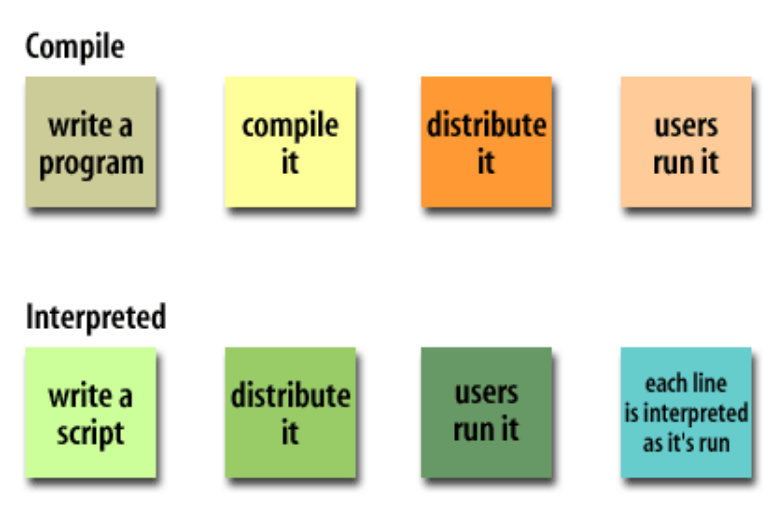
\includegraphics[width=0.5 \textwidth]{cvsi} 
\caption{Compiled Vs. Interpreted}
\end{figure}
}

\section{Setting up Environment}
\subsection{Installing python}
\begin{frame}[fragile]
  \frametitle{On Linux \small{(Ubuntu/Mint or similar)}}
  \begin{minted}{bash}
    $ sudo apt-get update 
    $ sudo apt-get upgrade 
    $ sudo apt-get install spyder python3-matplotlib
    $ sudo apt-get install  python3-scipy python3-pandas
\end{minted}
\end{frame}


\frame{
  \frametitle{On Windows}
  \begin{itemize}
  \item Download and install Anaconda
    \end{itemize}
      \hspace{1em}\textcolor{brown}{ \large{OR}}
      \small
  \begin{itemize}
    \item Download and install Winpython
    \end{itemize}
} 

\section{Python Basics}
\begin{frame}[fragile]
  \frametitle{Hello world and comments}
  \begin{columns}
  \hspace{-2em}\begin{column}{5cm}
  \begin{minted}{python}
  print("Hello World.")

  
  print("Hi")  # this prints "Hi" 

  
  ''' Everything within this is comment.
  This doesn't get evaluated.
  It's all comments!
  '''
  print("hi")
  \end{minted}
  \end{column}
  \begin{column}{5cm}
   \hspace{5em} $\leftarrow$    Hello World \\ 
    \vspace{2em}
    \hspace{5em}$\leftarrow$    inline  \\
    \vspace{3em}
    \hspace{5em}$\leftarrow$    multi-line \\ 
    \vspace{4em}
  \end{column}
 \end{columns}
 
\end{frame}

\begin{frame} [fragile]
  \frametitle{Usual Operations}
  \begin{minted}{python}
   + - * /            # basic arithmetic 
   //                 # integer division
   ++ --              # increment
   += -+ *=           # 
   **                 # power
   ==  != <= >= < >   # comparision
 \end{minted}
\vspace{2em}
\emph{Order of Operation matters!}
\end{frame}

\begin{frame} [fragile]
  \frametitle{Variables \& Data types}
\begin{minted}{python3}
     age = 5               # integer
     height = 123.2        # float
     college = "SXC"       # string
     isAlumni = True       # boolean

\end{minted}
\end{frame}

\begin{frame}[fragile]
  \frametitle{Strings}
\begin{minted}{python3}
   name = "John Doe"
   sentence = "My name is " + name +"."

   print(sentence, end=".")

   multiLine = ''' This is a
   string with multiple
   lines in it '''
\end{minted}
  \pause
  \textcolor{brown}{How would you print :  He said "I'm Lucky" ?} 
  \pause
  \begin{minted}{python3}
   print("He said \"I'm Lucky\"")  
   ''' \ is a way to escape special meaning (aka
      escape sequence) '''
\end{minted}
  \vspace{.5em}
\end{frame}

\begin{frame}[fragile]
  \frametitle{Strings}
\textbf{Some useful string methods: }
\begin{minted}{python3}
     .split()
     .replace("," , ".")
     .find()
     .count()
     .isalnum()
     .isalpha()
     .isdigit()
     .strip()
     
\end{minted}
\end{frame}


\begin{frame}[fragile]
  \frametitle{Taking inputs: }
\textbf{}
\begin{minted}{python3}
age = input("Enter your age: ")
print("Wow, you've been around for", age, "years!")
\end{minted}

\textbf{What if i enter characters and not digits?}

\end{frame}



\begin{frame}[fragile]
  \frametitle{Lists}
  \begin{itemize}
  \item collection of items
  \item could be heterogenous
  \item mutable
  \end{itemize}
  \vspace{2em}
\begin{minted}{python3}
shopping_list = ['tomatoes', 'potatoes', 'apples', 'juice', 'guava']

print("First item:", shopping_list[0])
\end{minted}
\end{frame}

\begin{frame}[fragile]
  \frametitle{Lists}
\textbf{List indexing and splicing}
\vspace{2em}
\begin{minted}{python3}

 list[1:3]    # from index 1 to 3 (excluding 3)

 list[:3]     # splicing
 list[2:]

 new_list = list[:]  # makes a copy
 list_2 = list       # giving another name

\end{minted}
\end{frame}

\begin{frame}[fragile]
  \frametitle{Lists}
\textbf{List inside of list}
\begin{minted}{python3}
matrix = [[1,2,3], [4,5,6], [7,8,9]]

print(matrix[1][0])       # this prints 6 !

matrix.append([10,11,12]) # now matrix is 4*3

matrix.insert(2,[2, 2, 3])  # inserts new row at index 2

a = [1, 4, 5]  
matrix = matrix + a         # combining to lists.
\end{minted}
\end{frame}

\begin{frame}[fragile]
  \frametitle{Lists}
\textbf{Some list useful methods: }
\begin{minted}{python3}
list.sort()
list.reverse()  # sorting

sorted()    # returns an iterable of sorted items

del(list[4])     # delete item at index 4
max() and min()  # first and last for non numbers)
\end{minted}
\end{frame}

\begin{frame}[fragile]
  \frametitle{Lists}
\textbf{Some \textit{more} list useful methods: }
\vspace{1em}
\begin{minted}{python3}
list = [3,1,4] 
len(list)      # length of the list (returns 3)

a = 3 in list  # a is True now
# item in list   evaluates to either true or false.

.find()
.search()
.replace()

\end{minted}
\end{frame}

\begin{frame}[fragile]
  \frametitle{Lists}
\vspace{1em}
\textbf{string are almost like lists !}
\end{frame}

\begin{frame}[fragile,fragile]
  \frametitle{Tuples}
\textbf{What are tuples?}
\begin{itemize}
\item list that cant be changed. 
\item fixed length, can't be appended or deleted.
\item comparable to struct in C
\item takes less memory and is faster 
\item list() and tuple() function to go back and forth between lists and tuple
\end{itemize}
\pause
\begin{minted}{python3}
point = (x, y)
student = (name, roll, enrollYr)

# they can be sliced just like lists
student[0]  # gives name of student
point[1]    # gives y co-ordinate of point

\end{minted}
\end{frame}

\begin{frame} [fragile]
  \frametitle{Dictionary}
  \begin{itemize}
  \item Dictionary stores key-value pair data \pause
  \item  also known as hash table, look-up table in other languages \pause
  \end{itemize}
  \vspace{1em}
\begin{minted}{python3}
        >>> 
        >>> capitals = {"Nepal": "Kathmandu",
                        "India": "New Delhi",
                        "Pakistan": "Islamabad"}

        >>> capital["Pakistan"]       # returns Islamabad
        >>> capital["France"] = "Rome"
        >>> del(capital["France"])    # as you'd expect
\end{minted}
\end{frame}

\begin{frame} [fragile]
  \frametitle{Dictionary}
\textbf{Some dictionary methods: }
 \begin{minted}{python3}
        >>> len(dict)
        >>> dict.keys()
        >>> dict.values()
 \end{minted}
\vfill
\end{frame}

\begin{frame} [fragile]
  \frametitle{Conditionals - if/else}
\textbf{When your code requires decision making based on conditions}
\vspace{1em}
 \begin{minted}{python3}

     >>> if age > 16:
     ...    print("You're old enough to drive")
     ... elif age > 25:
     ...    print("You're old enough to get married")
     ... else:
     ...     print("You're not old enough to drive or get married.")
 
\end{minted}
\vspace{1em}
\textbf{Python also has keywords like: and, or, not}
\vspace{1em}
\end{frame}




% \section{Section no.3} 
% \subsection{Tables}
% \frame{\frametitle{Tables}
% \begin{tabular}{|c|c|c|}
% \hline
% \textbf{Date} & \textbf{Instructor} & \textbf{Title} \\
% \hline
% WS 04/05 & Sascha Frank & First steps with  \LaTeX  \\
% \hline
% SS 05 & Sascha Frank & \LaTeX \ Course serial \\
% \hline
% \end{tabular}}


% \frame{\frametitle{Tables with pause}
% \begin{tabular}{c c c}
% A & B & C \\ 
% \pause 
% 1 & 2 & 3 \\  
% \pause 
% A & B & C \\ 
% \end{tabular} }


% \section{Section no. 4}
% \subsection{blocs}
% \frame{\frametitle{blocs}

% \begin{block}{title of the bloc}
% bloc text
% \end{block}

% \begin{exampleblock}{title of the bloc}
% bloc text
% \end{exampleblock}


% \begin{alertblock}{title of the bloc}
% bloc text
% \end{alertblock}
% }

% \section{Section no. 5}
% \subsection{split screen}

% \frame{\frametitle{splitting screen}
% \begin{columns}
% \begin{column}{5cm}
% \begin{itemize}
% \item Beamer 
% \item Beamer Class 
% \item Beamer Class Latex 
% \end{itemize}
% \end{column}
% \begin{column}{5cm}
% \begin{tabular}{|c|c|}
% \hline
% \textbf{Instructor} & \textbf{Title} \\
% \hline
% Sascha Frank &  \LaTeX \ Course 1 \\
% \hline
% Sascha Frank &  Course serial  \\
% \hline
% \end{tabular}
% \end{column}
% \end{columns}
% }

% \subsection{Pictures} 
% \frame{\frametitle{pictures in latex beamer class}
% \begin{figure}
% \includegraphics[scale=0.5]{PIC1} 
% \caption{show an example picture}
% \end{figure}}

% \subsection{joining picture and lists} 

% \frame{
% \frametitle{pictures and lists in beamer class}
% \begin{columns}
% \begin{column}{5cm}
% \begin{itemize}
% \item<1-> subject 1
% \item<3-> subject 2
% \item<5-> subject 3
% \end{itemize}
% \vspace{3cm} 
% \end{column}
% \begin{column}{5cm}
% \begin{overprint}
% \includegraphics<2>{PIC1}
% \includegraphics<4>{PIC2}
% \includegraphics<6>{PIC3}
% \end{overprint}
% \end{column}
% \end{columns}}

\end{document}